\begin{figure}[h] 
\centering 
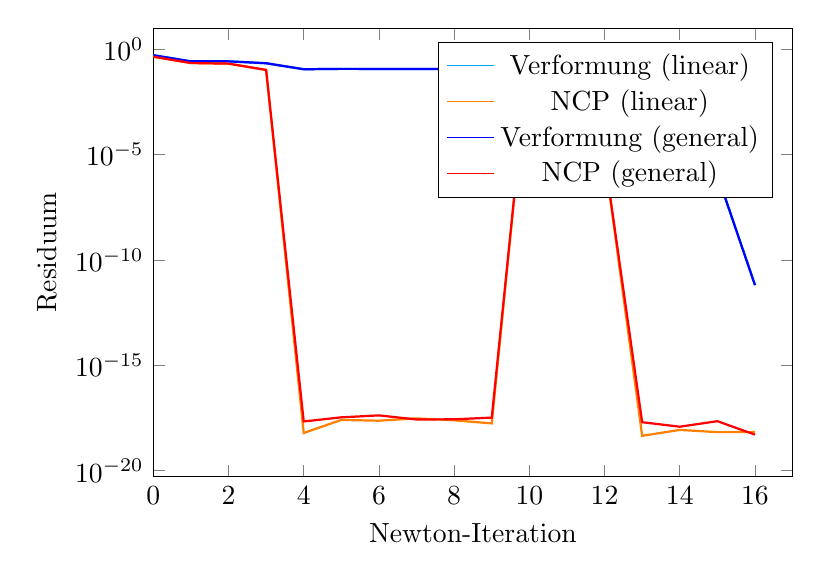
\begin{tikzpicture}[every plot/.append style={thick}] 
\begin{axis}[ 
label style={font=\normalsize}, 
xlabel={Newton-Iteration}, 
ylabel={Residuum}, 
xmin=0, xmax=17, 
ymode=log, 
ymin=0, ymax=10, 
width=0.8\textwidth, 
height=0.6\textwidth, 
legend pos=north east, 
legend style={cells={align=left}}, 
grid style=dashed, 
] 
\addplot[ 
color=cyan, 
] 
coordinates { 
(0, 5.24e-01)(1, 2.68e-01)(2, 2.68e-01)(3, 2.18e-01)(4, 1.13e-01)(5, 1.18e-01)(6, 1.17e-01)(7, 1.15e-01)(8, 1.15e-01)(9, 1.15e-01)(10, 5.21e-01)(11, 4.41e-01)(12, 7.57e-02)(13, 9.50e-03)(14, 4.51e-04)(15, 1.09e-06)(16, 6.45e-12)}; 
\addlegendentry{Verformung (linear)} 
\addplot[ 
color=orange, 
] 
coordinates { 
(0, 4.46e-01)(1, 2.23e-01)(2, 2.09e-01)(3, 1.05e-01)(4, 6.20e-19)(5, 2.58e-18)(6, 2.37e-18)(7, 3.06e-18)(8, 2.47e-18)(9, 1.77e-18)(10, 1.31e+00)(11, 1.09e+00)(12, 8.02e-06)(13, 4.55e-19)(14, 8.66e-19)(15, 6.80e-19)(16, 6.84e-19)}; 
\addlegendentry{NCP (linear)} 
\addplot[ 
color=blue, 
] 
coordinates { 
(0, 5.24e-01)(1, 2.68e-01)(2, 2.68e-01)(3, 2.18e-01)(4, 1.13e-01)(5, 1.18e-01)(6, 1.17e-01)(7, 1.15e-01)(8, 1.15e-01)(9, 1.15e-01)(10, 5.21e-01)(11, 4.41e-01)(12, 7.57e-02)(13, 9.50e-03)(14, 4.51e-04)(15, 1.09e-06)(16, 6.45e-12)}; 
\addlegendentry{Verformung (general)} 
\addplot[ 
color=red, 
] 
coordinates { 
(0, 4.46e-01)(1, 2.23e-01)(2, 2.09e-01)(3, 1.05e-01)(4, 2.18e-18)(5, 3.43e-18)(6, 4.24e-18)(7, 2.71e-18)(8, 2.76e-18)(9, 3.33e-18)(10, 1.31e+00)(11, 1.09e+00)(12, 8.02e-06)(13, 2.01e-18)(14, 1.23e-18)(15, 2.25e-18)(16, 5.16e-19)}; 
\addlegendentry{NCP (general)} 
\end{axis} 
\end{tikzpicture} 
\caption{Residuen des Stoffgesetzes 'St.Venant' mit Hinderniss 'Spitze' und 2178 Freiheitsgraden für die Verschiebung.} 
\label{fiq:St.Venant_Spitze_level4} 
\end{figure} 
